\documentclass[11pt]{scrartcl}
\usepackage{graphicx}
\usepackage[margin=12mm]{geometry}
\usepackage{sectsty}
\usepackage{mathtools}
\usepackage{subfigure}
\sectionfont{\fontsize{12}{10}\selectfont}

\begin{document}
\title{ECSE 526-Artificial Intelligence}
\subtitle{Assignment 2 - Music Classifier}
\author{Alexandre Coulombe - 260801407}
\date{February 19th, 2020}
\maketitle



\section{Assumptions about the data when using a Gaussian distribution}

There are a few assumptions about the data that are made when using the linear Gaussian distribution model. First of all, the data is assumed to have a normal/Gaussian distribution with mean $\mu$ and variance $\sigma^2$. For the case of this assignment, the 12 features of the data would form a 12-dimensional Gaussian distribution over the data of a certain genre. The distribution would need to be symmetric about its mean $\mu$ to form the Gaussian distribution. 

A second assumption is that the data forms distributions that are distinguishable from each other. This would mean that the distribution of the data of different classes does not overlap significantly with another class's Gaussian distribution. This would allow the linear Gaussian model to identify the various classes in the data set.

In addition, we assume that we can model the 12-dimensional distribution using the mean and the covariance matrix of the class on new queries to be able to identify its class. This would mean that an entire data set would be represented by only the mean and the covariance matrix of the class, which would be suitable if the data follows a Gaussian distribution. 

\section{When to apply a linear Gaussian model}

A Gaussian model is best used when the data follows a Gaussian distribution. For example, this can be data sets that form a ``bell shaped curved" in n-dimensions. An example of this would be the grade distribution on a test. In a case like the previous, the Gaussian classifier would be able to fit the data set and be able to predict the output of a query. Due to it using the same distribution model as the data set, the Gaussian classifier would be better suited for predicting query outputs than other classifiers.

In the case where the assumptions listed in the previous section are not meet, the Gaussian model is not suitable. This can be the case on data sets that have asymmetry around the mean, or have multiple peaks along the distribution. Another case where the Gaussian classifier would not work well is when the data of multiple classes are very similar to each other. This would mean that two classes would have distribution with a large amount of overlap, making classification difficult. Also, Gaussian would not be well suited for data sets where the data of a distribution is far apart or when outliers are present. This would stretch the distribution and make it ignore the outlier cases which would make the model classify outlier queries wrong.

\section{Best value of k for the K-Nearest Neighbors classifier}

The K-Nearest Neighbours (K-NN) algorithm is a non-parametric learning algorithm that searches for the $k$ points nearest to the query point and use the labels of the neighbouring points in a majority vote to determine what the label of the query should be. The value of $k$ determines the accuracy of the algorithm. For the case of $k=1$, the algorithm would be using the closest point to the query and taking its label, which is a case of overfitting the data set. In this case, the accuracy would suffer from outliers in the data set providing the wrong label to the query point. By increasing the value of $k$, we would reach a case of underfitting where we would use a large portion of the data set and the label that is most common in the data set is the label given to the query points. This would reduce the accuracy as well.

By the two extremes demonstrated previously, a value of $k$ between the extremes would provide the highest accuracy. In the case of the data set for the music classifier, it is found experimentally that the best value of $k$ to use in the K-NN is 11 or 12. Multiple values of $k$ yielded different accuracies with $k=11$ and $k=12$ yielding the highest with an accuracy of $63.12\%$. The accuracy for other values of $k$ can be observed in Figure \ref{fig:F1}.

%Add figure to document
\begin{figure}[ht]
\centering	
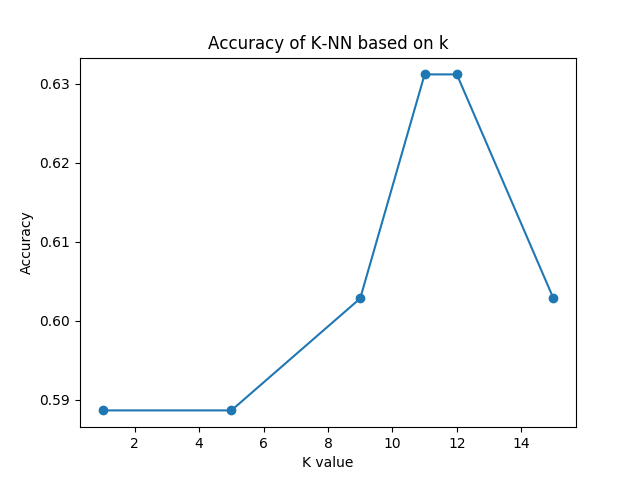
\includegraphics[scale=0.75]{Figure_1.png}	
\caption{Accuracy of the K-Nearest Neighbors algorithm based on the selected value of $k$}
\label{fig:F1}
\end{figure}

\section{Best Music Classifier}

For this assignment, the linear Gaussian, the K-NN and its variant weighted K-NN were implemented and used on the data set. The linear Gaussian had the worst performance out of the three algorithms with an accuracy of $26.95\%$ on the Kaggle test set. This is because the data set does not follow the assumptions stated for using a Gaussian model. By looking at the histograms of each of the features in the training set, illustrated in Figure \ref{fig:F14}, we can see that the features do not all follow a symmetry about the mean of the class's training data. It must also be noted that, more importantly, the distributions have a large overlap between each other. In this case, the distribution with the highest probabilities in a region, namely \textit{rnb} for the cluster of densities, is the class that the linear Gaussian goes for, while those of different shapes, namely \textit{classical} and \textit{pop}, are used for data that doesn't match the cluster of density around \textit{rnb}.  

%Add figure to document
\begin{figure}[ht]
\centering
\subfigure[Feature 1]{\label{fig:F2}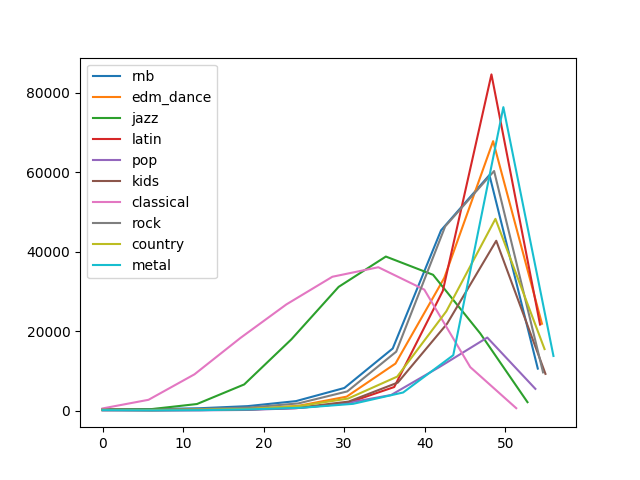
\includegraphics[width=0.24\textwidth, height=4cm]{Figure_2.png}}	
\subfigure[Feature 2]{\label{fig:F3}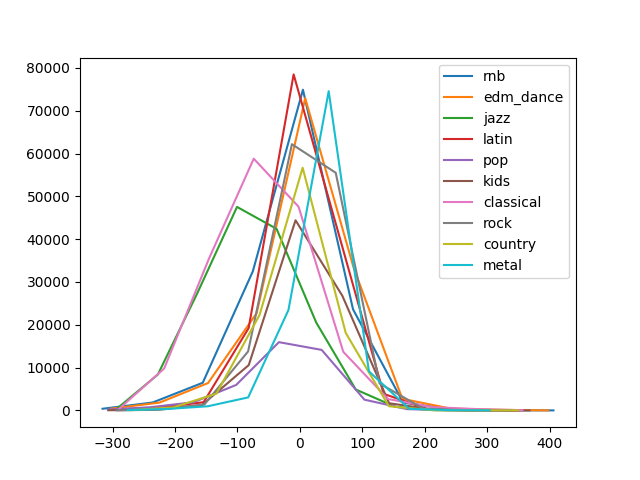
\includegraphics[width=0.24\textwidth, height=4cm]{Figure_3.png}}	
\subfigure[Feature 3]{\label{fig:F4}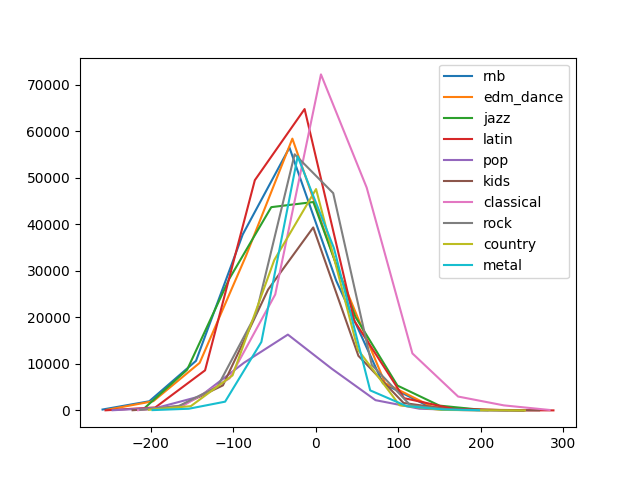
\includegraphics[width=0.24\textwidth, height=4cm]{Figure_4.png}}
\subfigure[Feature 4]{\label{fig:F5}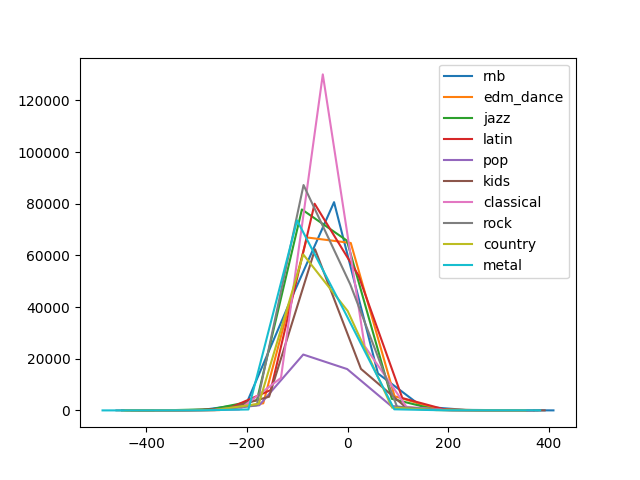
\includegraphics[width=0.24\textwidth, height=4cm]{Figure_5.png}}		
\subfigure[Feature 5]{\label{fig:F6}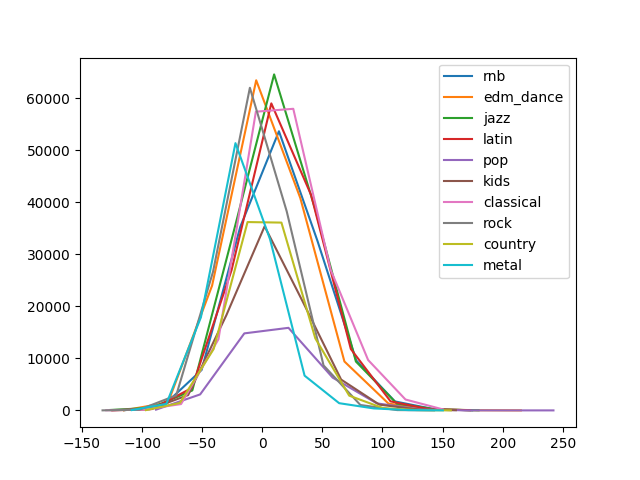
\includegraphics[width=0.24\textwidth, height=4cm]{Figure_6.png}}
\subfigure[Feature 6]{\label{fig:F7}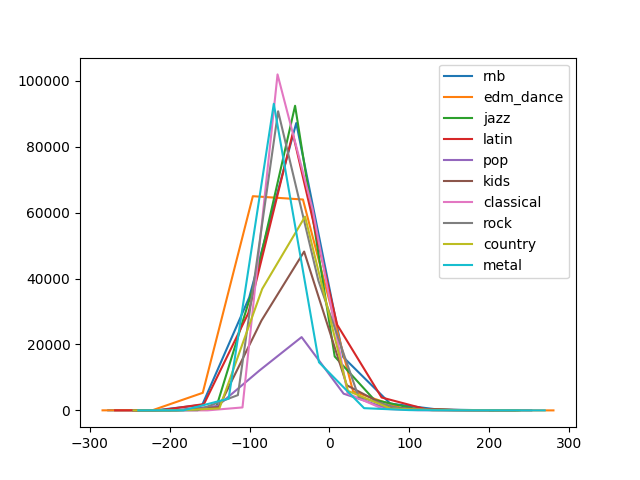
\includegraphics[width=0.24\textwidth, height=4cm]{Figure_7.png}}
\subfigure[Feature 7]{\label{fig:F8}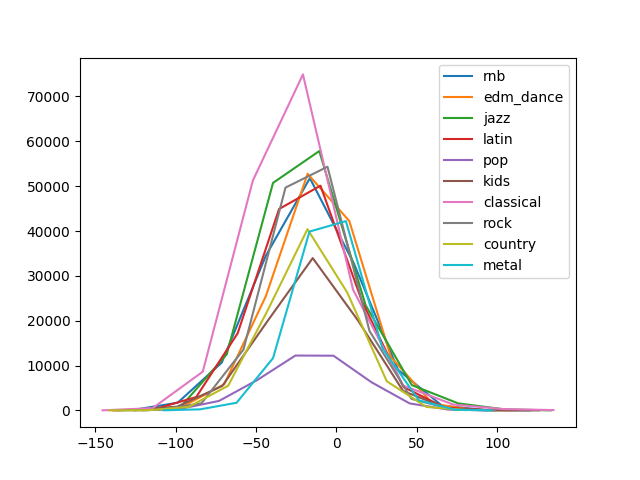
\includegraphics[width=0.24\textwidth, height=4cm]{Figure_8.png}}
\subfigure[Feature 8]{\label{fig:F9}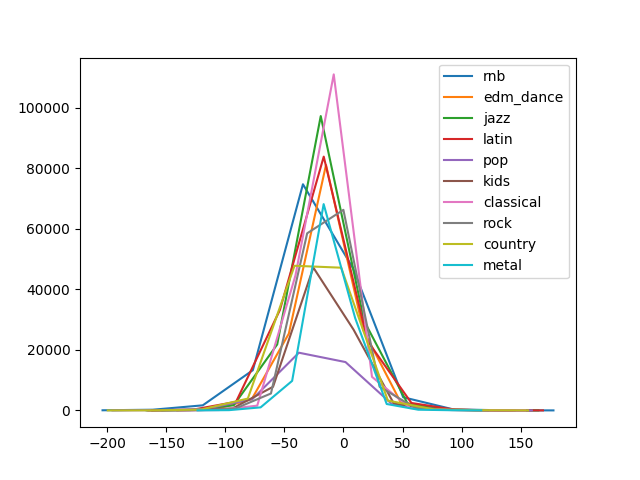
\includegraphics[width=0.24\textwidth, height=4cm]{Figure_9.png}}	
\subfigure[Feature 9]{\label{fig:F10}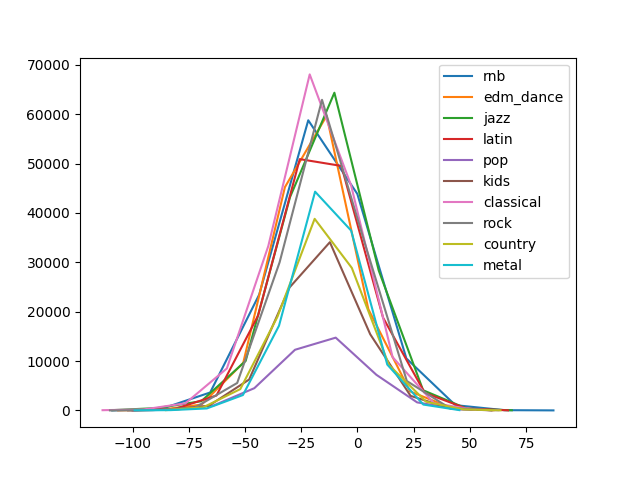
\includegraphics[width=0.24\textwidth, height=4cm]{Figure_10.png}}
\subfigure[Feature 10]{\label{fig:F11}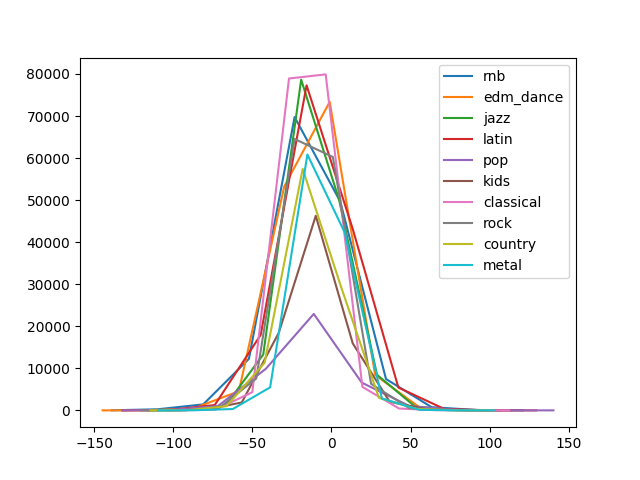
\includegraphics[width=0.24\textwidth, height=4cm]{Figure_11.png}}
\subfigure[Feature 11]{\label{fig:F12}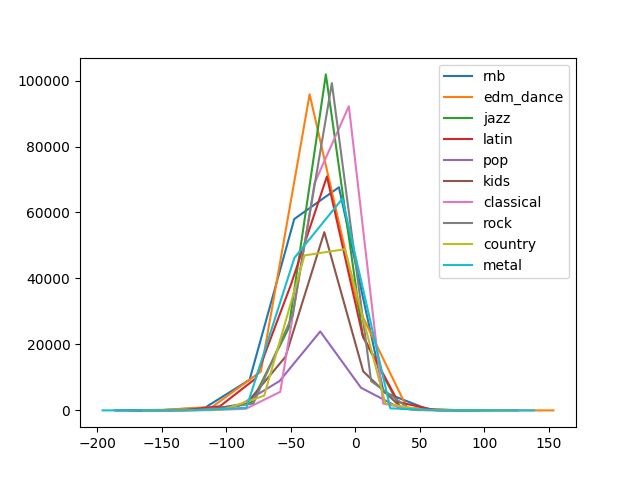
\includegraphics[width=0.24\textwidth, height=4cm]{Figure_12.png}}
\subfigure[Feature 12]{\label{fig:F13}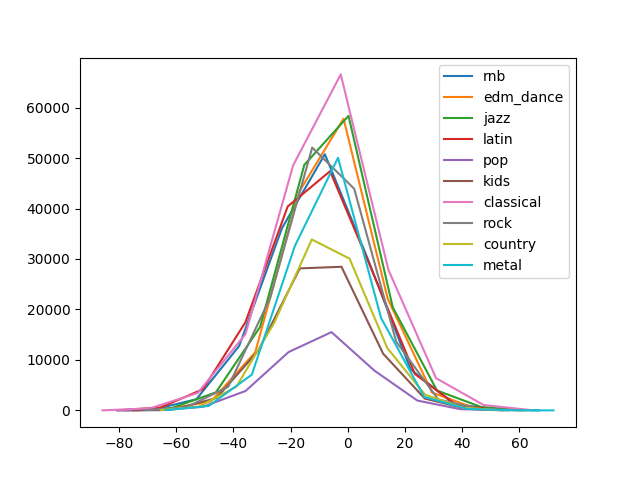
\includegraphics[width=0.24\textwidth, height=4cm]{Figure_13.png}}
\caption{Histograms of the 12 features of the data set}
\label{fig:F14}
\end{figure}

K-NN performs much better than the linear Gaussian model of the data. This is due to the K-NN algorithm retaining all the information of the training set instead of parameterizing the training data to be represented by a certain number of parameters and using the parameters to  classify new query features into a class. In the case of the linear Gaussian, a $12\times 12$ covariance matrix and a $12\times 1$ mean vector represent the entire training set of a genre, which loses information about the data about outliers or asymmetry. In addition, the overlapping of all of the distributions makes the parameters of the covariance matrix and the mean vector of each class become almost the identical and end up pointing to the same class. However, in the K-NN algorithm, all the training set examples are kept and used to determine the class of a new query point. Since no information is lost and there are no assumptions on the data, the K-NN would have a higher accuracy than the linear Gaussian, which is the case. The K-NN has more than double the accuracy of the linear Gaussian even with various values of $k$ seen in Table \ref{table:T0}. The best accuracy of the K-NN was $63.12\%$ with $k=11$ and $k=12$ as stated before. 

\begin{table}[ht]
\centering
 \begin{tabular}{||c c | c c||} 
 \hline
 \multicolumn{2}{|c|}{K-NN} & \multicolumn{2}{|c|}{Weigthed K-NN}\\ 
 \hline
 $k$ value & Accuracy(\%) & $k$ value & Accuracy(\%) \\ [0.5ex] 
 \hline
 1 & 58.865 & 11 & 63.829 \\ 
 \hline
 5 & 58.865 & 13 & 65.258\\
 \hline
 9 & 60.283 & 15 & 64.539\\
 \hline
 11 & 63.120 & 21 & 63.829 \\
 \hline
 12 & 63.120 & - & - \\
 \hline
 15 & 60.283 & - & - \\ [1ex] 
 \hline
\end{tabular}
\caption{Accuracy of K-NN and weighted K-NN based on various values of $k$}
\label{table:T0}
\end{table} 

The K-NN was improved by taking into account the distance between the query point and the training set point in order to give a weight to each of the training set point labels. This modification results in the weighted K-NN algorithm where points closer to the query point have a higher weight, because they are so much more like the query point, than points further away, which are less like the query point. This prevents points from being wrongly labelled because the label belonging to the nearest neighbours that are very far away outnumber the label belonging to the nearest neighbours that are very close to the query. An example would be having $k=15$ where 5 nearest neighbours that are very close to each other have class A and 10 nearest neighbours that are very far away from each other have class B. In K-NN, the prediction would give class B, but, for weighted K-NN, the very close points would outweigh the far away points classing the query as class A. This change increased the accuracies on the test set compared to the K-NN, but not by very much as seen in Table \ref{table:T0}. Thus, the weighted K-NN algorithm is the best classifier for the music classifier out of the linear Gaussian, K-NN, and weighted K-NN algorithms. There is the possibility that another algorithm has a much higher accuracy, but it has not been explored during this assignment.

\end{document}